\section{Tangential Acceleration and Centripetal Acceleration}

\begin{comment}
This lab is new in fall 2019 by Matt Trawick.  I ran this for the very first time in my class this fall, and it seemed
to work fine.  The students also said it went okay.  

This lab is meant to address a topic my students have generally found confusing.  I

\end{comment}

\makelabheader %(Space for student name, etc., defined in master.tex or labmanual_formatting_commands.tex)

\bigskip

\textbf{Activity 1: Drawing Vectors}

The picture below shows a top view of a car speeding up while taking a curve on a road. 

(a)  Use graphical techniques (no calculations) to draw a vector representing the change in velocity $\Delta \vv{v}$ during the time shown.

\hspace{1.0in}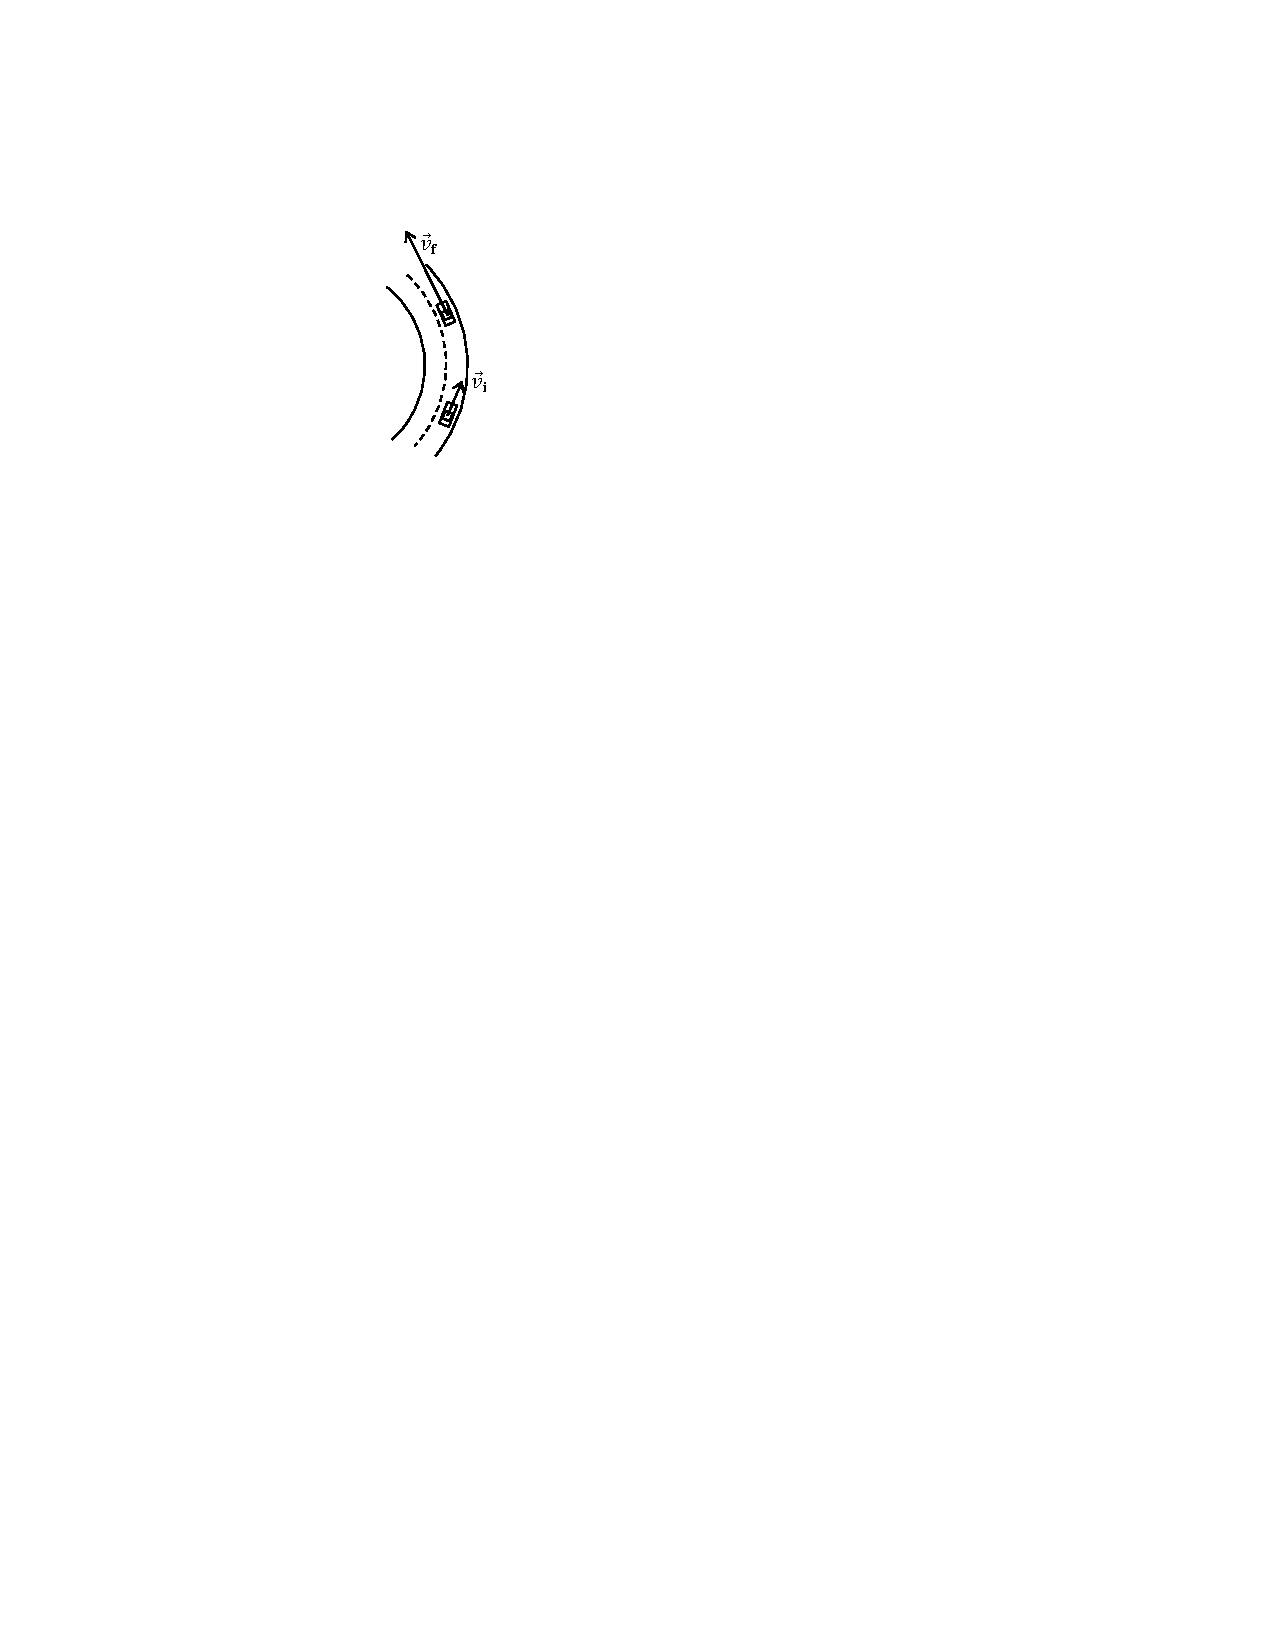
\includegraphics{tangential_and_centripetal_acc/curve1.pdf}

(b) Does the average acceleration $\vv{a}_{\rm avg}$ during this time point exactly towards the center of the curve?
\answerspace{0.3in}


(c) You may have done previous exercises
that involved a car driving on a circular track, in which the average acceleration always pointed towards the center of the curve.  
\iflabelexists{vector_addition_exercises}{(See Lab \ref{vector_addition_exercises}, for instance.)}{}
Why is the case pictured above different?
\answerspace{0.4in}

\textbf{Activity 2: An Example with Numbers}

(a) Suppose you are driving north on a straight road.  You accelerate uniformly from rest to a speed of 15~m/s over a time $\Delta t = 5$ seconds.  What is the magnitude and direction of your accleration $\vv{a}$ during this time?  Also draw your acceleration vector $\vv{a}$ on the picture below.

\hspace{1.0in}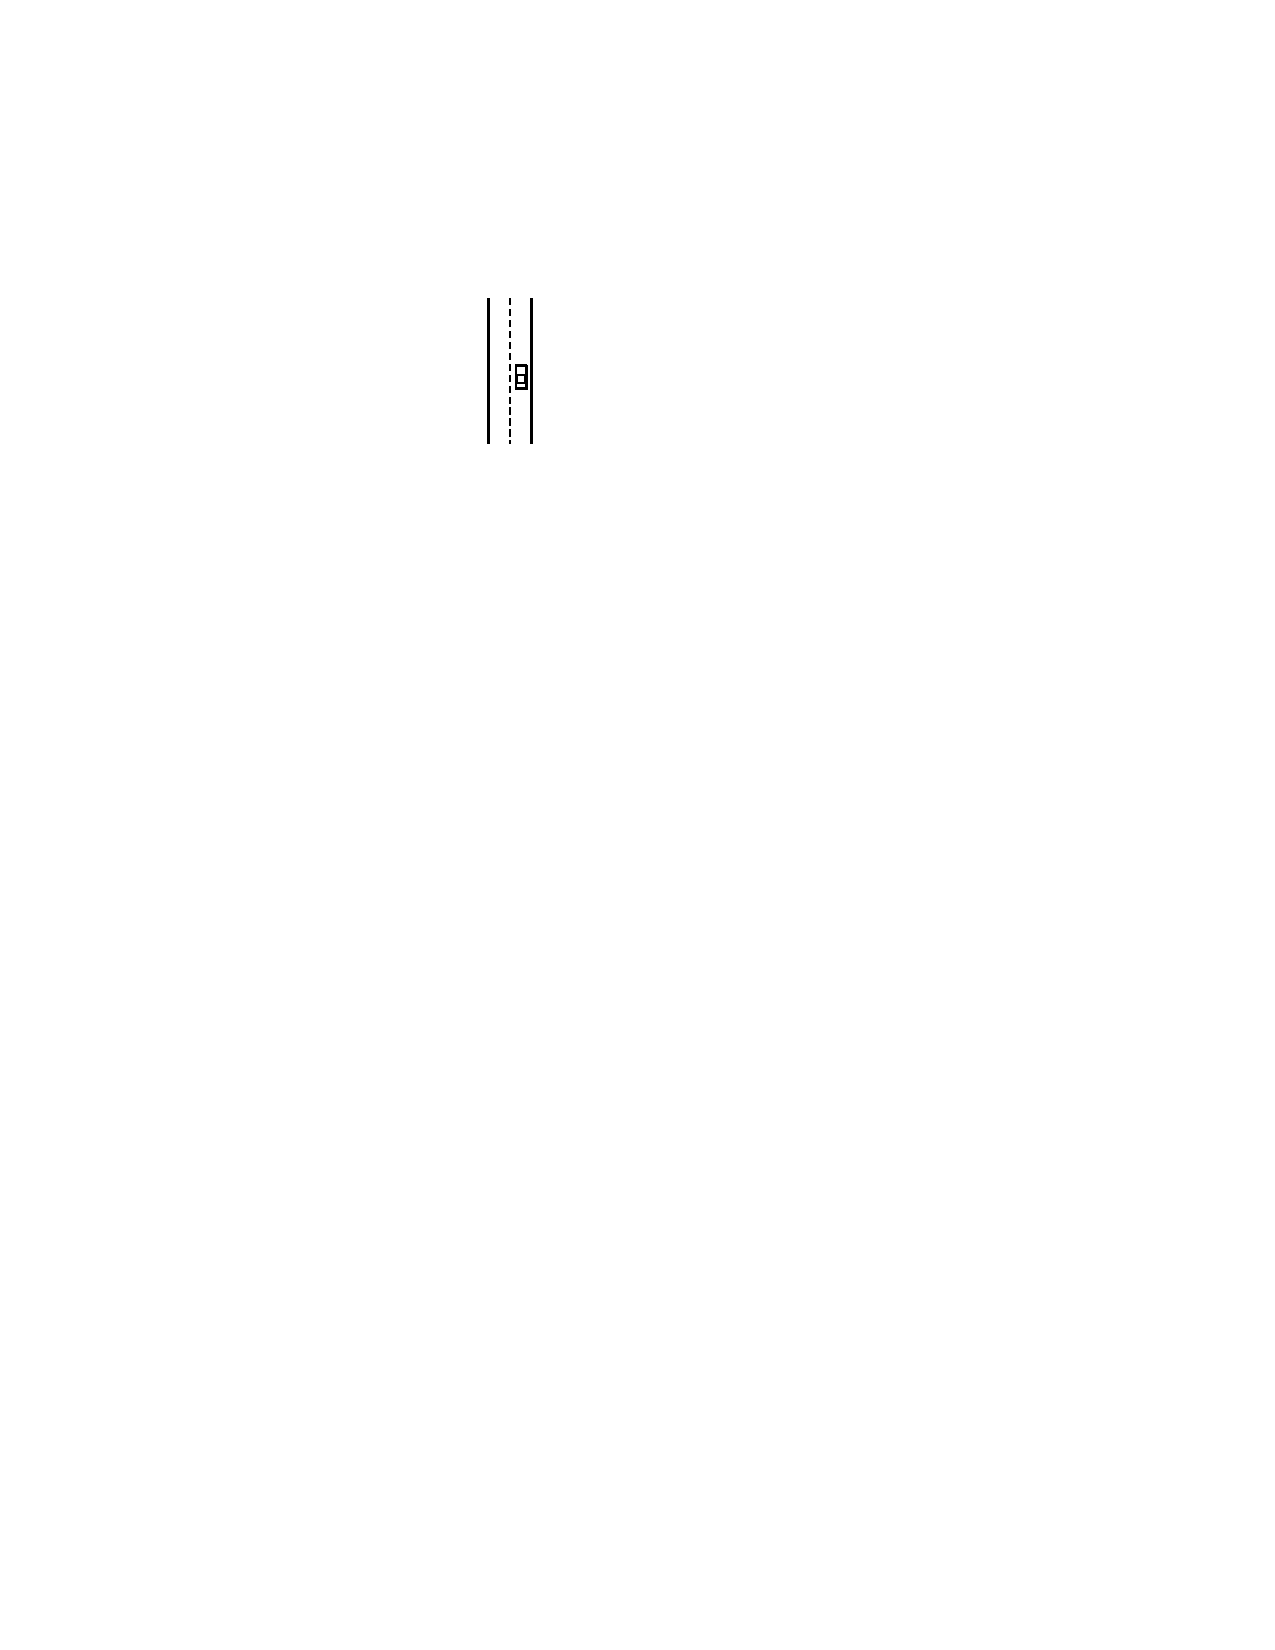
\includegraphics{tangential_and_centripetal_acc/straight.pdf} 
\hspace{0.1in}
\parbox{1.5 in}{\raggedright{\textit{(causing acceleration with the gas pedal...)}}}

(b) Now suppose you are driving at a constant speed $v=10$~m/s around a curve of radius $R=25$~m.  What is the magnitude and direction of your acceleration $\vv{a}$ at exactly the moment pictured below?  Also draw your acceleration vector $\vv{a}$ on the picture.

\hspace{1.0in}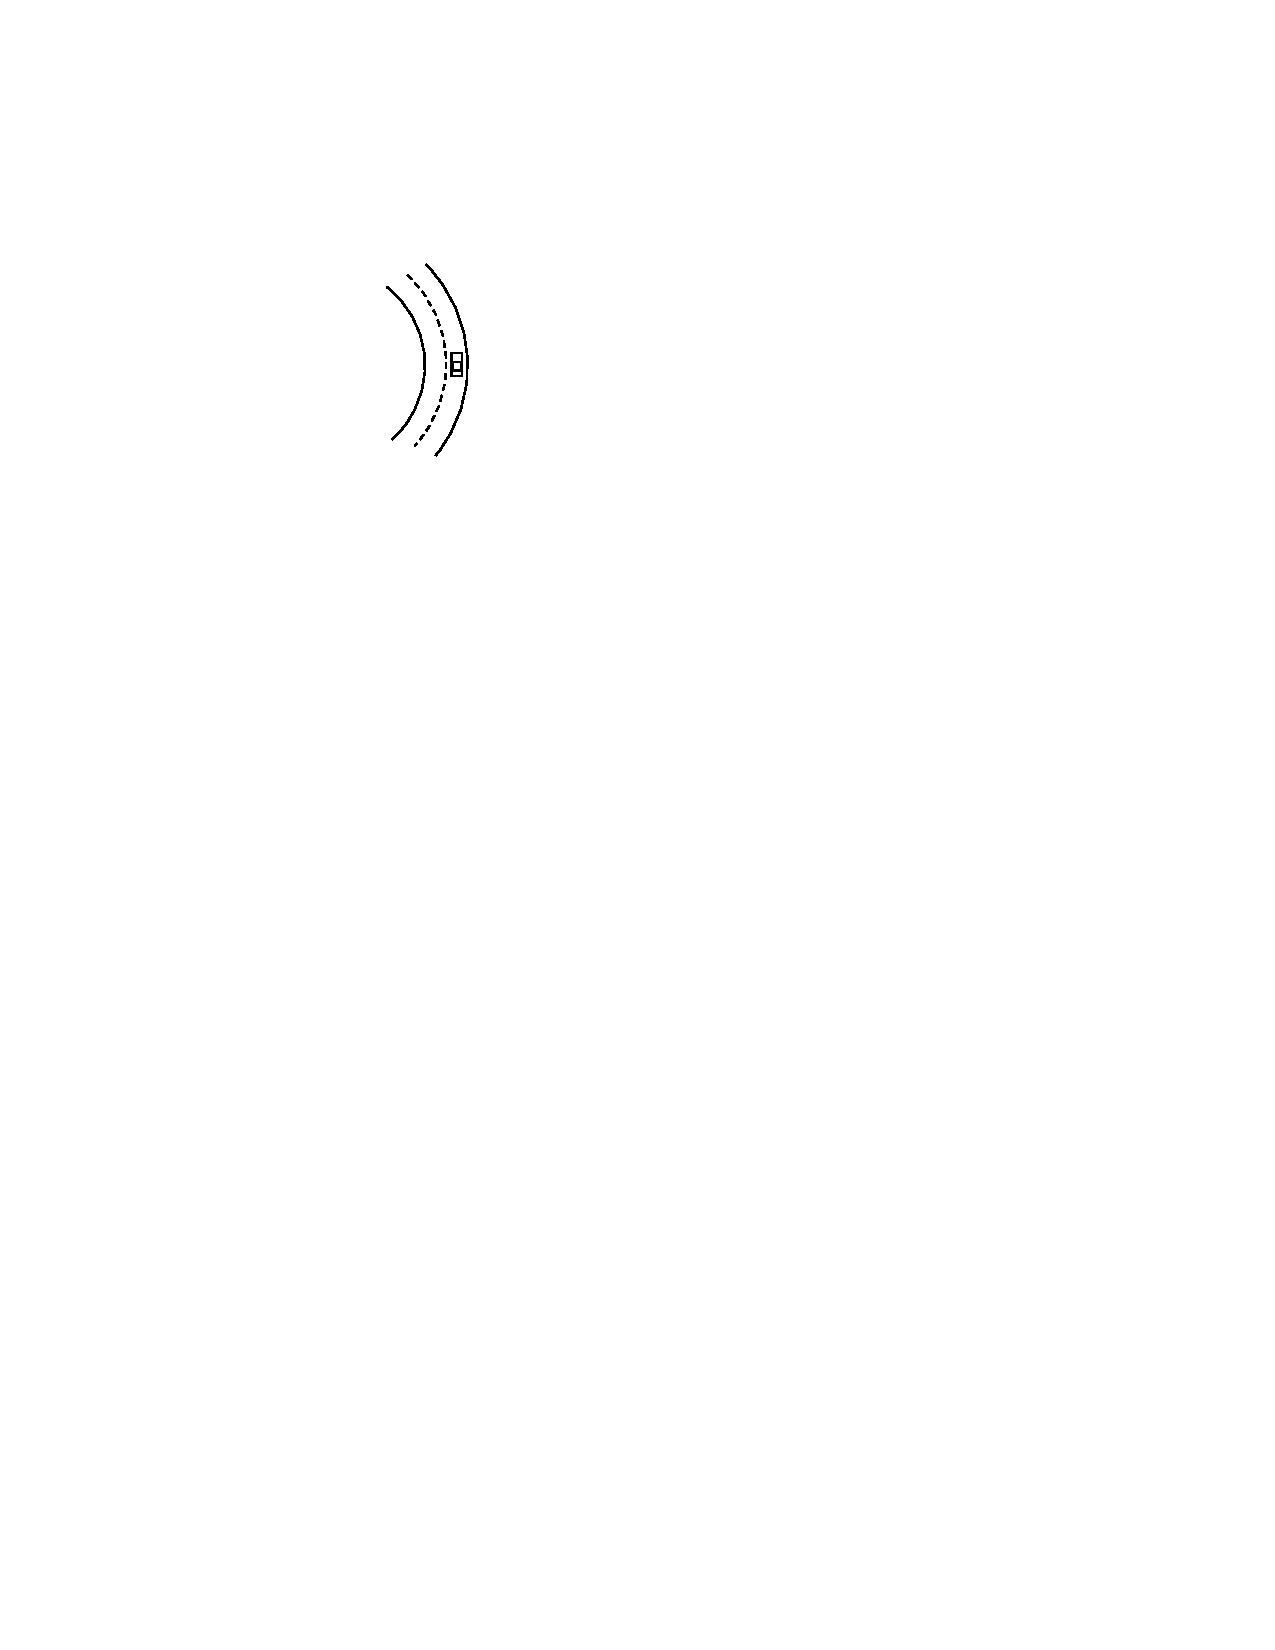
\includegraphics{tangential_and_centripetal_acc/curve2.pdf} 
\hspace{-0.2in}
\parbox{2.0 in}{\raggedright{\textit{(causing acceleration \linebreak with the steering wheel...)}}}

%\pagebreak[3]
(c) Finally, suppose that you 
increase your speed just like you did in part (a), but you do it \textit{while} taking the same curve in the road as you did in part (b).   You are now combining the accelerations from parts (a) and~(b), doing both at the same time.  Draw your acceleration vector $\vv{a}$ on the picture below.  \textit{(Hint: what does it mean to ``combine'' two acceleration vectors?)}

\hspace{1.0in}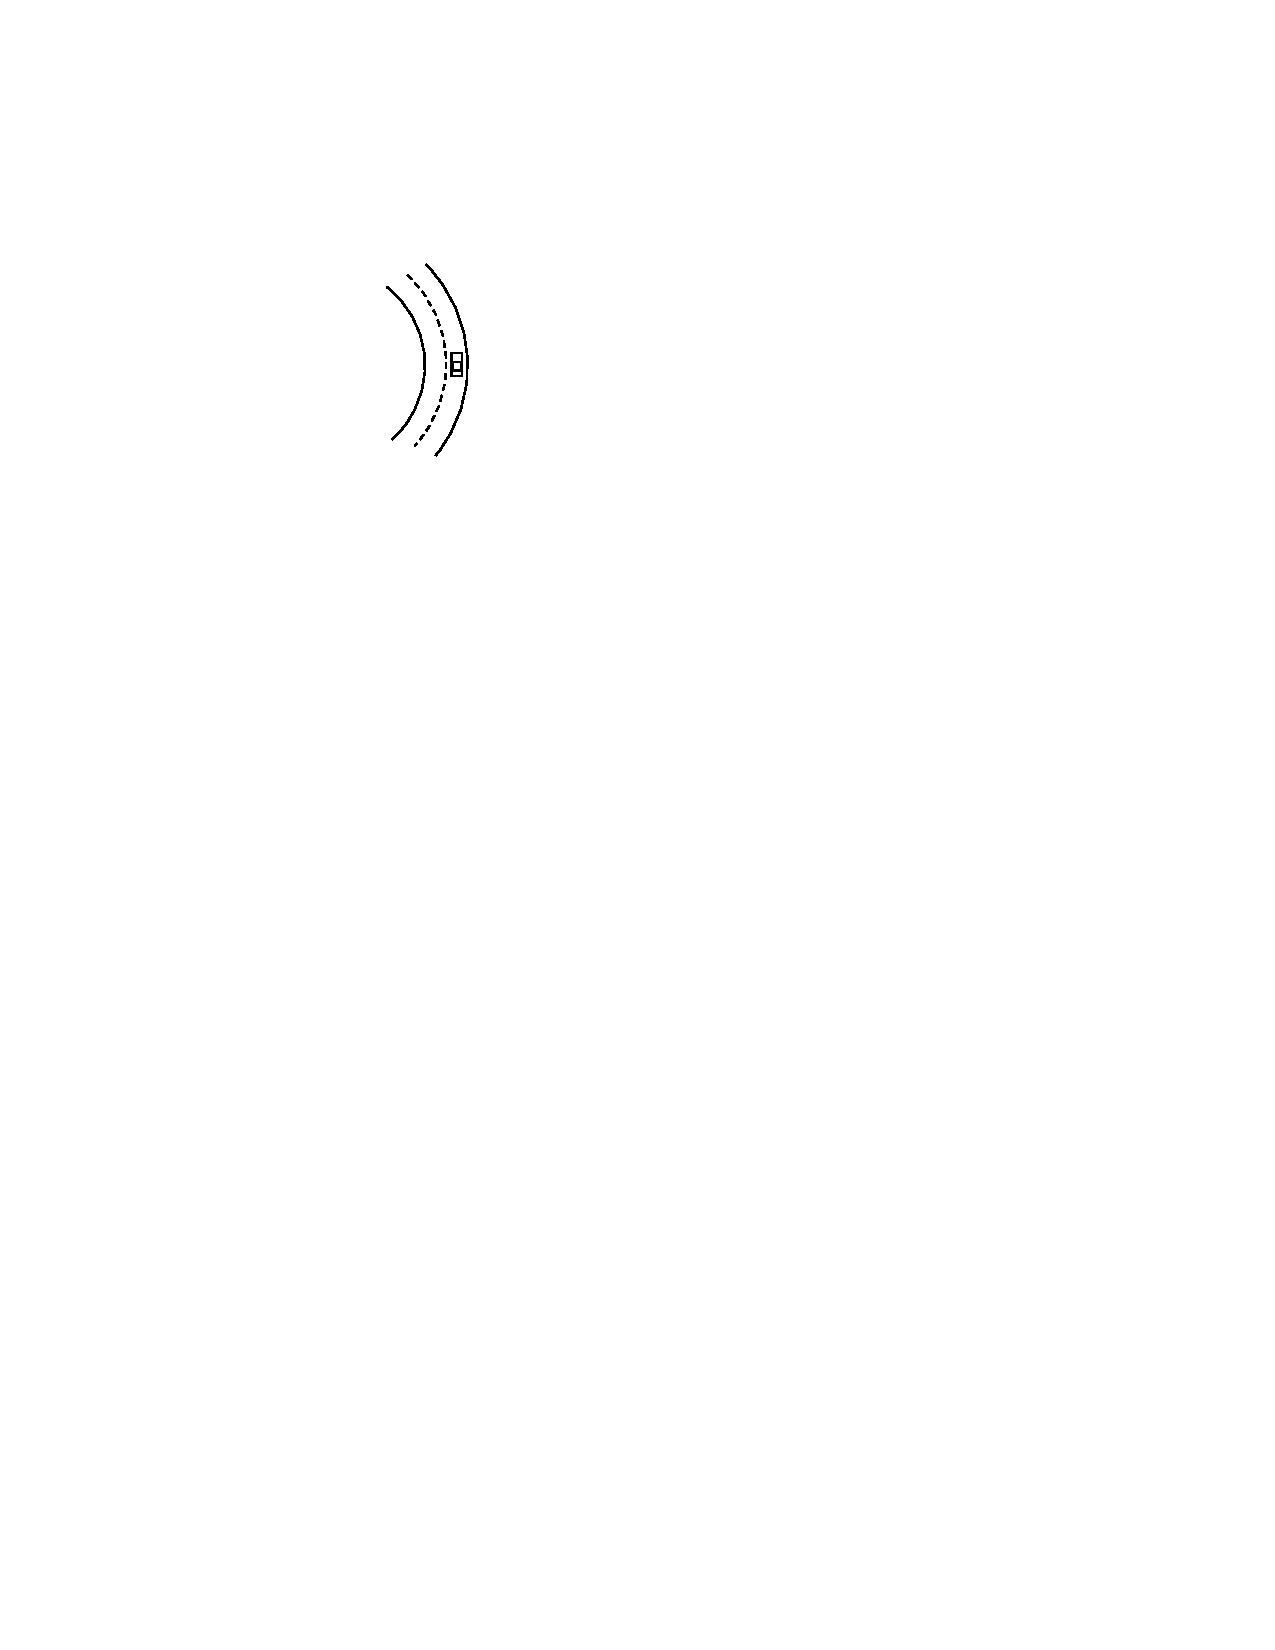
\includegraphics{tangential_and_centripetal_acc/curve2.pdf} 
\hspace{-0.2in}
\parbox{2.0 in}{\raggedright{\textit{(causing acceleration \linebreak 
with \textbf{both} the gas pedal \linebreak 
\textbf{and} the steering wheel...)}}}

\bigskip
Let's use the same numbers as we did before: you increased your speed from from 0~m/s to 15~m/s over $\Delta t = 5$~s, and at the moment shown in the picture above, you happen to have a speed of exactly $v=10$~m/s.

(d) What is the \textit{tangential} component $a_t$ of your acceleration?  (That is, the component of your acceleration vector $\vv{a}$ that is along your direction of motion.)
\answerspace{0.4in}

(e) What is the \textit{centripetal} component $a_c$ of your acceleration?  (That is, the component of your acceleration vector $\vv{a}$ that is towards the center or the curve.)
\answerspace{0.4in}

(f) What are the magnitude and direction of your acceleration $\vv{a}\,$?
\answerspace{1.5in}

%(g) In what direction is the net force $\vv{F}_{\rm NET}$ on your car at this time?
%[This question isn't really needed, and without it the lab can fit nicely with kinematics.]
%\answerspace{0.5in}



